\documentclass[sigconf]{acmart}
\settopmatter{printacmref=false} % Removes citation information below abstract
\renewcommand\footnotetextcopyrightpermission[1]{} % removes footnote with conference information in first column
\pagestyle{plain}

\usepackage{graphicx}
\usepackage{balance}  % for  \balance command ON LAST PAGE  (only there!)
\usepackage{pgfplots}
\usetikzlibrary{patterns}
\usepackage{pgfplotstable}
\usetikzlibrary{arrows, decorations.markings}
\usepackage[binary-units=true]{siunitx}
\sisetup{
     per-mode = symbol
}
\DeclareSIUnit{\void}{\relax}
\usepackage{fancyvrb}
\usepackage{multicol}
\usepackage{listings}
\usepackage{booktabs}
\usepackage{algorithm}
\usepackage[noend]{algpseudocode}
\makeatletter
\renewcommand{\ALG@name}{Pseudocode}
\usepackage{amsmath}
\usepackage{wrapfig}
\usetikzlibrary{matrix}
\usepgfplotslibrary{groupplots}
\pgfplotsset{compat=newest}
\usepackage{dblfloatfix}
\usepackage{newfloat}
\usepackage{makecell}
\usepackage{cancel}
\usepackage{varwidth}
\usepackage{bbding}
\usepackage{enumitem}
\usepackage[caption=false]{subfig}
\usepackage{mathtools}
\renewcommand{\contentsname}{Referenzen}
\renewcommand{\refname}{Referenzen}

\DeclarePairedDelimiter\abs{\lvert}{\rvert}
\interfootnotelinepenalty=10000

%fix for algo2e in regular float
\makeatletter
\newcommand{\removelatexerror}{\let\@latex@error\@gobble}
\makeatother


\lstdefinestyle{mkc}{
  belowcaptionskip=1\baselineskip,
  breaklines=true,
  frame=L,
  xleftmargin=\parindent,
  language=C,
  showstringspaces=false,
  basicstyle=\footnotesize\ttfamily,
  keywordstyle=\bfseries\color{green!40!black},
  commentstyle=\itshape\color{purple!40!black},
  stringstyle=\color{orange},
}

\pgfplotscreateplotcyclelist{barplot-cyclelist}{
    black, fill=white\\% postaction={pattern color=black,   pattern=fill}\\%
    black, fill=black!50\\% postaction={pattern color=black,   pattern=fill}\\%
    black,  postaction={pattern color=black,      pattern=north east lines}\\%
    black,  postaction={pattern color=black,   pattern=crosshatch dots}\\%
}

\begin{document}


\title{Deduplikation}

\author{Daniel Stefan Heinz-Eugen Klose}
\affiliation{
  \institution{TU Dortmund University}
}
\email{daniel-stefan.klose@udo.edu}

%\titlenote{}
%\subtitle{}

\begin{abstract}
  Ein wichtiger Teil des ETL-Prozesses ist die Deduplikation.
  In dieser Ausarbeitung werde ich mich genauer mit dem Thema
  der Deduplikation
  befassen. Es werden mehrere Metriken vorgestellt, an denen
  man Duplikate erkennen kann.
  Des Weiteren werde ich eine Methode vorstellen, mit der man
  diese effizient implementieren kann.

\end{abstract}

\maketitle

\section*{Problem}
In einem OLTP-System sind die Daten meist "schmutzig". Das bedeutet, 
dass das ein Großteil der Daten auch nach wie vor mit der Hand von
einzelnen Personen in das Datenbank-System eingetragen werden. 

Bei diesen eingetragen
passieren verschiedene Fehler. Ein Fehler davon ist, das ein Eintrag 
falsch geschrieben ist bzw. mit verschiedenen Schreibweisen des
selben Eintrags in dem 
Datenbank-System zu finden ist. Ein Beispiel dafür ist die 
Schreibweise für Dortmund. Ein Mitarbeiter eines Unternehmens 
macht unabsichtlich einen Schreibfehler und trägt Dortmond als 
Verkaufsort eines Produkts.

Dies führt dazu, dass nach der Überführung der Daten in ein
Datawarehouse dieser Verkauf nicht zu den Verkäufen des Standortes 
Dortmund gehört und damit auch nicht bei den Aggregationen mit 
eingerechnet wird. Hier kommt die Deduplikation im ETL-Prozess 
ins Spiel.

\section*{Lösung}
Das Finden und Zusammenführen von solchen Duplikaten wird im 
ETL-Prozess auch Deduplikation genannt. Bei der einfachsten Form 
für das Finden von Duplikaten vergleichen wir, mit einem vorher 
festgelegtem Maß jedes Wort mit jedem anderen und führen diese 
zusammen welche unterhalb eines bestimmten Thresholds liegen.

Im weiteren Verlauf dieser Arbeit werden wir sehen, dass dies eine sehr
ineffiziente Lösung ist und schauen uns weitere Alternativen an.


\subsection*{Vergleichsmaße}
Als Erstes wollen wir uns verschiedene Vergleichsmaße ansehen, 
wie auch die verschiedenen Ansätze dieser.

Das wohl einfachste Maß für die Gleichheit zweier Zeichenketten
ist die sogenannte \emph{Editierdistanz} \cite[Vgl. S. 2] {cohen2003comparison}, 
welche auch als \emph{Levenshtein-Distanz} bezeichnet wird.
Die Editierdistanz misst, wie viele Operationen es braucht, 
um den einen String in den anderen zu transformieren. 
Die Operationen lauten \emph{erstzen}, wobei ein Zeichen
durch ein weiteres ersetzt wird, \emph{einfügen}, wobei ein
Zeichen in einen String eingefügt wird und \emph{löschen}, 
wobei ein Zeichen gelöscht wird. Um dies zu implementieren 
machen wir Gebrauch von dem Konzept der 
\emph{dynamischen Programmierung}. Der Algorithmus ist
in Pseudocode \ref{alg:editdistance} zu sehen 
\cite[Vgl. S. 223] {bille2005survey}.

  \begin{algorithm}
    \begin{algorithmic}[1]
      
      \Procedure{distance}{$u$, $v$}
      \State {$m := \abs{u}$}
      \State {$n := \abs{v}$}
      \State {decalre $d[0..m, 0..n]$}
      \For{$i$ from $0$ to $m$}
        \State $d[i,0] := i$
      \EndFor
      \For{$i$ from $0$ to $n$}
        \State $d[0,i] := i$
      \EndFor

      \For{$i$ from $1$ to $m$}
        \For{$j$ from $1$ to $n$}
          \If {$u[i] = v[j]$}
            \State {$cost := 0$}
          \Else
            \State {$cost := 1$}
          \EndIf
          \State \begin{varwidth}[t]{\linewidth}
            $d[i,j] := min ($\par
              \hskip\algorithmicindent $d[i-1,j]+1, $\par
              \hskip\algorithmicindent $d[i,j-1]+1$\par
              \hskip\algorithmicindent $d[i-1,j-1] + cost)$
            \end{varwidth}
        \EndFor
      \EndFor
    
      \Return{$d[m,n]$}
      \EndProcedure
      
    \end{algorithmic}
    \caption{Editierdistanz mit dynamischer Programmierung}
    \label{alg:editdistance}
    \end{algorithm}

Als weiters Maß für das Finden von Duplikaten ist die
\emph{Jaccard Similarity} \cite[Vgl. 4.1.1]{theobald2008spotsigs}. 
Diese misst die Ähnlichkeit von Mengen. Da wir aber keine Mengen 
vergleichen sonders Strings, machen wir einen
kleinen Trick und überführen unsere Strings in Mengen, indem wir
jeweils zwei aufeinanderfolgende Zeichen des Strings zu einem Element
der Menge machen. Zum Beispiel wird aus $"Sweet"$ dann
$\{"Sw", "we", "ee", "et" \}$. Damit können wir auch Strings vergleichen.
Das Vergleichen selber geschieht mit der Formel:
$$\frac{\abs{S_1 \cap S_2}}{\abs{S_1 \cup S_2}}$$
Als Beispiel vergleichen wir \emph{Sweet} und \emph{Sweat}.

\begin{gather*}
  \frac{
    \abs{\{"Sw", "we", "ee", "et" \} \cap \{"Sw", "we", "ea", "at" \}}
  }{
    \abs{\{"Sw", "we", "ee", "et" \} \cup \{"Sw", "we", "ea", "at" \}}
  }
  = \\
  \frac{
    \abs{\{"Sw", "we"\}}
  }{
    \abs{\{"Sw", "we", "ee", "et", "ea", "at" \}}
  }
  = 
  \frac{1}{3}
\end{gather*}

Neben diesen Maßen existieren weiter, welche sich an der
Aus-sprache von Worten orientiert. Hierfür ist der Soundex 
\cite[Vlg. S. 5]{elmagarmid1} sowie Metaphone 
\cite[Vlg. S. 5]{elmagarmid1} ein Beispiel.
Beim Soundex wird das erste Zeichen beibehalten und die folgenden
Zeichen werden durch die jeweilige Nummer ersetzt. 
Andere Zeichen werden entfernt. Doppelt aufeinander 
folgende Zahlen werden auf eine Reduziert.
Es werden maximal drei Nummern verwendet. Falls weniger vorhanden sind,
werden sie mit Nullen aufgefüllt. Die Zeichen werden
wie folgt esetzt:


\[ f(n) =
  \begin{cases}
    1      & \text{falls } n \in \{b,f,p,v\}\\
    2      & \text{falls } n \in \{c,g,j,k,q,s,x,z\}\\
    3      & \text{falls } n \in \{d,t\}\\
    4      & \text{falls } n \in \{l\}\\
    5      & \text{falls } n \in \{m,n\}\\
    6      & \text{falls } n \in \{r\}\\
    -     & \text{sonst }\\
  \end{cases}
\]




\subsection*{Vergleichsmatix}
Um jeden String mit jedem anderen zu vergleichen Stellen wir eine
sogenannte Vergleichsmatrix auf. Haben wir eine List $l$ an Strings
bekommen wir eine Matrix $d$ mit $\abs{l\times l}$ Elementen. Da alle
Vergleichsmaße kommutativ sind und der Vergleich mit sich Selbs
irrelevant ist, müssen wir jedoch nur die Einträge oberhalb der
Diagonalen von $d[0,0]$ bis $d[\abs{l}, \abs{l}]$ betrachten.
Dies ist in Abbildung \ref{abb:matrix} dargestellt. Hierbei
sind nur die roten Zellen Interessant und müssen berechnet werden.

\begin{figure}[htbp]
  \centering
  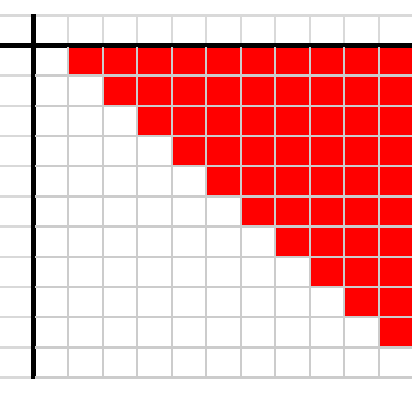
\includegraphics{table.pdf}
  \caption{Volle Vergleichsmatix}
  \label{abb:matrix}
\end{figure}

Dabei sieht man auch sofort das Problem der vollen Vergleichsmatrix.
Es müssen sehr viele Vergleiche gemacht werden. Bei $n$
Strings müssen
$$\frac{n^2}{2} - n$$
Vergleiche gemacht werden.
Bei $1000$ verschiedener
Elemente müssen $499000$ bei $10000$ schon $49990000$ Vergleiche
gemacht werden. Dies wird sehr schnell ineffiziente.

Die effizientere Lösung ist hier das Blocking \cite[Vlg. S. 11]{elmagarmid1}.
Beim Blocking berechnen wir nicht die gesamte
Vergleichsmatrix, sondern wir teilen die Liste der Strings
in Blöcke auf. Die Vergleiche finden nun nur noch in diesen
Blöcken statt, welches in Abbildung \ref{abb:matrixblock} zu sehen ist,
oder es wird ein Fenster einer bestimmten Blockgröße über die
Diagonale geschoben und Vergleiche werden nur innerhalb
dieses Fensters gemacht.

\begin{figure}[htbp]
  \centering
  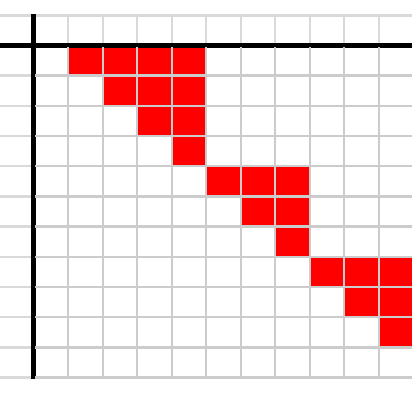
\includegraphics{table2.pdf}
  \caption{Vergleichmatrix mit Blocking}
  \label{abb:matrixblock}
\end{figure}

Wenn wir jedoch nur die Liste strikt in $n$
Teile aufteilen verlieren wir an Genauigkeit, da wir
manche Strings, welche eigentlich die selbe Bedeutung haben,
nicht vergleichen.
Um das zu verhindern, teilen wir nicht einfach in $n$
Blöcke, sondern wir sortieren die Strings anhand von
bestimmten Kriterien. Strings eines bestimmen Kriteriums kommen
einen Block bzw. werden anhand dieser sortiert \cite[Vlg. S. 11]{elmagarmid1}.
Diese Kriterien-Blöcke verhindern, dass
ähnliche Strings in einen Block kommen
und verglichen werden.
Es gibt mehrere Strategien Kategorien zu wählen. Diese
kommt immer auf den Kontext des Strings bzw. der Entity 
im OLAP-Systems an.
Eine Strategie ist es nach dem Anfangszeichen zu
sortieren, da dort meist kein Fehler gemacht wird.
Eine bessere Strategie ist jedoch sich die Entity,
die diesen String beschreibt, genauer anzusehen,
um dort eine Eigenschaft zu finden, welche sehr
Fehlertolerant und 2 String mit gleicher Bedeutung
dieselbe Eigenschaft haben.
Nehmen wir zum Beispiel das Deduplizieren von
Straßennamen. Hier könnte eine sinnvolle
Eigenschaft sein einen Präfix der
Postleitzahl zu nehmen, da diese oft richtig
Eingegeben werden und zwei Straßennamen mit selber
Bedeutung immer dieselbe Postleitzahl haben.

Wenn wir die $n$ Strings in $b$ gleich große Blöcke
einteilen erhalten wir eine Laufzeit von
$$\frac{1}{2} (\frac{n^2}{b}-n)$$
Durch das Aufteilen in Blöcken nach verschiedenen
Eigenschaften reduzieren wir die Wahrscheinlichkeit,
dass wir manche Duplikate nicht finden.

Eine weitere Erweiterung davon wäre, wenn man diese
Auf-teilung in Blöcke und das Finden von Duplikaten
mehrmals mit verschiedenen Eigenschaften durchführt
\cite[Vlg. S. 11]{elmagarmid1}.
Dadurch sinkt die Wahrscheinlichkeit von Duplikaten
im Endresultat noch einmal.

\section*{Zusammenfassung}
Alles zusammen ist die Deduplikation ein essentieller 
Bestandteil des ETL-Processes.
Jedoch muss eine durch den Kontext bedingte Strategie entwickelt
werden um Duplikate sicher und effizient finden zu
können. Hierbei ist zuerst die Wähl des Vergleichsmaß
entscheidend. Des Weiteren muss eine Fehlertolerante
und mit der Bedeutung übereinstimmende Eigenschaft
gefunden werden, um die String ideal zu sortieren bzw. 
in Blöcke einteilen zu können.

\bibliographystyle{abbrv}
\bibliography{acmart}

\end{document}

